\section{Architektura systemu}
\label{sec:architektura-systemu}
Projekt jest zbudowany w oparciu o architekturę klient-serwer (rys. \ref{fig:system-architecture-basic}, \ref{fig:system-architecture}). Rolę serwera pełni płytka Terasic DE1-SOC, a klientem jest komputer PC. Komunikacja odbywa się przez kabel USB, przez który tunelowany jest sygnał UART.

\begin{figure}[!h]
\centering
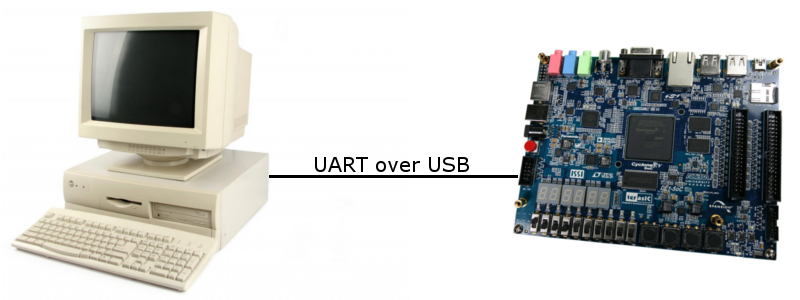
\includegraphics[width=6in]{pictures/system-architecture-basic.png}
\caption{Architektura klient-serwer systemu (na zdjęciu laptop Dell XPS 13 \cite{laptop} oraz płytka Terasic DE1-SOC \cite{plytka})}
\label{fig:system-architecture-basic}
\end{figure}

\begin{figure}[!h]
\centering
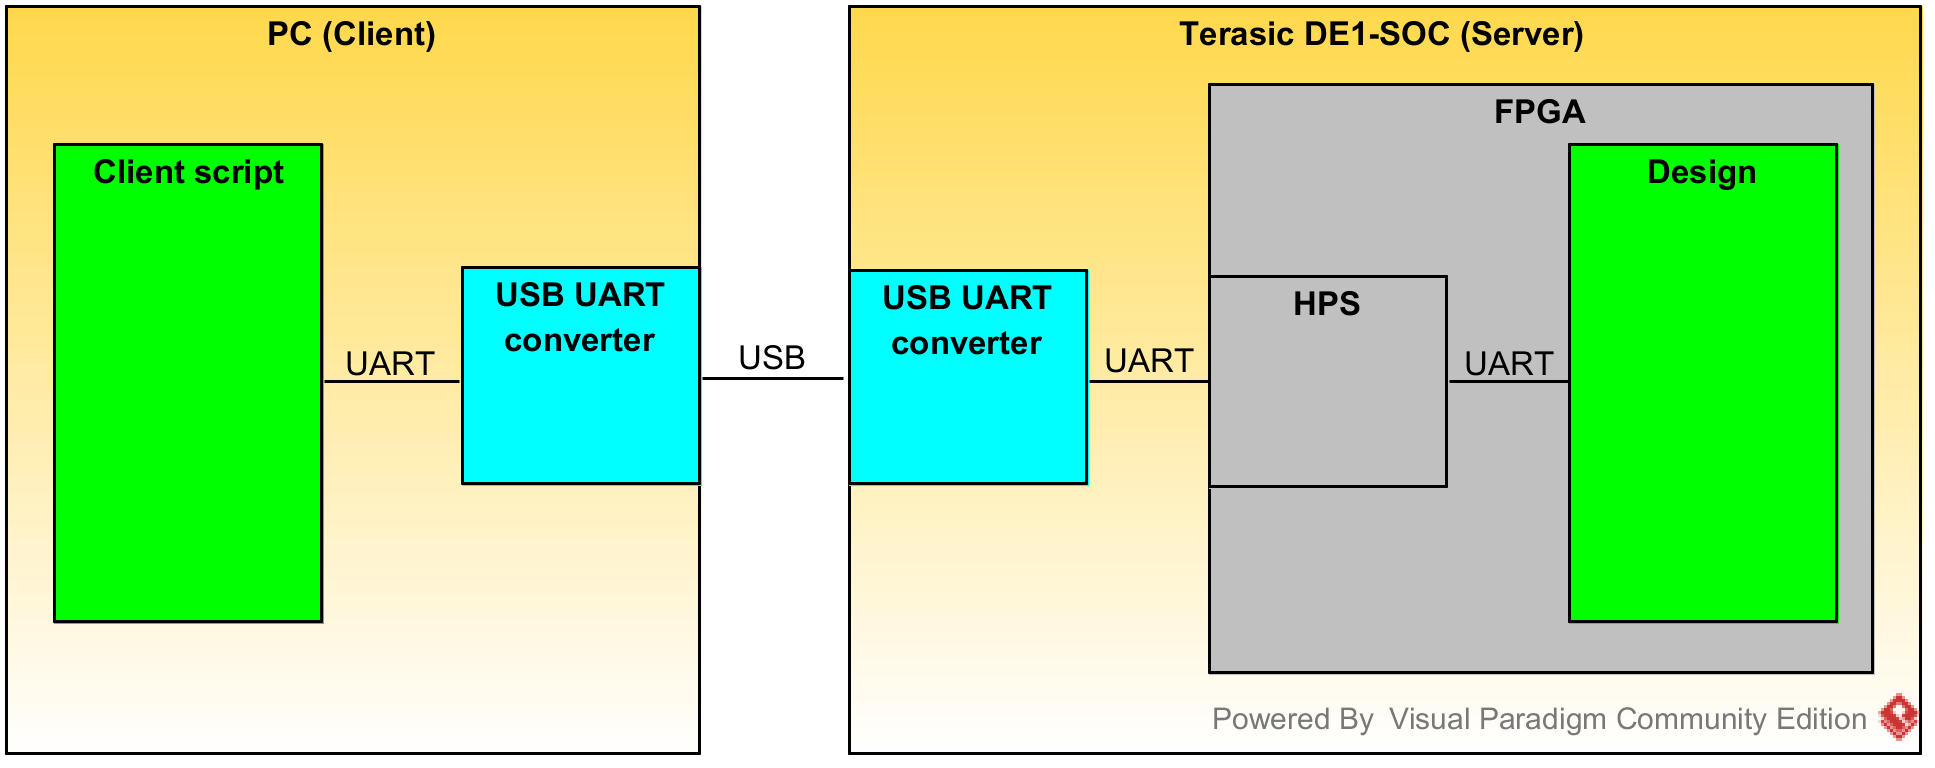
\includegraphics{pictures/system-architecture.png}
\caption{Części składowe systemu}
\label{fig:system-architecture}
\end{figure}

Serwer (płytka Terasic DE1-SOC) wyposażony jest w układ Altera Cyclone V SoC 5CSEMA5F31C6, który zawiera programowalną część FPGA oraz posiada zintegrowany procesor ARM (HPS - ang. \textit{hard processor system}). FPGA jest zaprogramowany tak, aby realizował komunikację UART oraz szyfrowanie i deszyfrowanie AES. Sygnały UART biegnące do układu konwertera USB-UART są podłączone do części HPS, w wyniku czego komunikacja między FPGA a konwerterem USB-UART musi zachodzić przez piny HPS, które zostały skonfigurowane tak aby było to możliwe (rozdz. \ref{sec:uart-qsys}).

Klientem jest komputer PC z systemem operacyjnym Ubuntu. Programem udostępniającym użytkownikowi funkcjonalność szyfrowania i deszyfrowania plików jest skrypt, który odpowiada za komunikację z serwerem wykonującym zlecona zadania.

Komunikacja między klientem a serwerem odbywa się przez kabel USB, którym tunelowany jest sygnał UART. Końcówką tunelu po stronie serwera jest konwerter UART-USB firmy FTDI. Po stronie klienta tunel obsługiwany jest przez wbudowany w system operacyjny sterownik, który umożliwia realizację komunikacji w sposób analogiczny do zwykłego portu szeregowego.


\subsection{Przebieg komunikacji}
\label{sec:przebieg-komunikacji}
Komunikacja między komputerem (klientem) a układem FPGA (serwerem) w celu zaszyfrowania informacji przebiega według schematu:
\begin{enumerate}[noitemsep]
\item Klient wysyła bajt ENC lub DEC wskazujący, czy dane mają być szyfrowane czy deszyfrowane.
\item Serwer odpowiada bajtem ACK jeśli odebrał bajt o wartości ENC lub DEC, NACK w innym przypadku.
\item Jeśli klient otrzymał NACK kończy działanie.
\item Klient wysyła blok zawierający 128 młodszych bajtów klucza oraz 2 bajty CRC16.
\item Serwer odpowiada ACK jeśli blok został przesłany poprawnie (suma kontrolna CRC16 bloku jest równa wartości odebranej), NACK w przeciwnym przypadku.
\item Jeśli klient otrzymał NACK, retransmituje blok oraz oczekuje na potwierdzenie. Retransmisja wykonywana jest do skutku.
\item Klient wysyła blok zawierający 128 starszych bajtów klucza oraz 2 bajty CRC16.
\item Serwer odpowiada ACK jeśli blok został przesłany poprawnie, NACK w przeciwnym przypadku.
\item Jeśli klient otrzymał NACK, retransmituje blok oraz oczekuje na potwierdzenie. Retransmisja wykonywana jest do skutku.
\item Klient wysyła blok zawierający wektor inicjalizacji oraz 2 bajty CRC16.
\item Serwer odpowiada ACK jeśli blok został przesłany poprawnie, NACK w przeciwnym przypadku.
\item Jeśli klient otrzymał NACK, retransmituje blok oraz oczekuje na potwierdzenie. Retransmisja wykonywana jest do skutku.
\item Klient wysyła pierwszy blok danych oraz 2 bajty CRC16.
\item Serwer odpowiada ACK jeśli blok został przesłany poprawnie, NACK w przeciwnym przypadku.
\item Jeśli klient otrzymał NACK, retransmituje blok oraz oczekuje na potwierdzenie. Retransmisja wykonywana jest do skutku.
\item Serwer szyfruje otrzymany blok, wysyła go oraz 2 bajty CRC16. Jednocześnie Klient wysyła kolejny blok do zaszyfrowania.
\item Serwer sprawdza sumę kontrolną CRC16 otrzymanego bloku i wysyła bajt ACK jeśli blok został otrzymany poprawnie lub NACK w przeciwnym przypadku. Jednocześnie klient postępuje analogicznie.
\item Jeśli odebrany przez serwer blok jest poprawny, oraz jeśli otrzymał od klienta bajt ACK, szyfruje otrzymany blok oraz odsyła go do klienta. W przeciwnym przypadku retransmituje poprzedni zaszyfrowany blok.
\item Jeśli odebrany przez klienta blok jest poprawny, oraz jeśli otrzymał od serwera bajt ACK, wysyła kolejny blok do zaszyfrowania. W przeciwnym wypadku retransmituje poprzedni blok.
\item Wymiana bloków zachodzi dopóki wszystkie informacje nie zostaną zaszyfrowane. O końcu transmisji decyduje klient. Po wysłaniu ostatniego bloku i odebraniu przedostatniego zaszyfrowanego bloku, jeśli zaszyfrowany blok zastał odebrany poprawnie, zamiast ACK wysyła FIN.
\item Serwer po odebraniu bajtu FIN szyfruje ostatni blok oraz odsyła go do klienta.
\item Jeśli klient otrzymał ostatni blok poprawnie wysyła bajt ACK oraz kończy działanie, w przeciwnym wypadku wysyła NACK.
\item Jeśli serwer otrzymał bajt ACK przechodzi do stanu oczekiwania na rozpoczęcie kolejnego procesu szyfrowania. W przeciwnym wypadku retransmituje ostatni zaszyfrowany blok oraz czeka na potwierdzenie. Retransmisja wykonywana jest do skutku.
\end{enumerate}

\begin{figure}[!h]
\centering
\begin{tikztimingtable}[timing/wscale=2.9]
  \textit{RX} & h d{ENC} h      1.5D{KEY\_LOW} h      1.5D{KEY\_HIGH} h      1.5D{INIT\_V} h      1.5D{D1\_PLAIN} h      1.5D{D2\_PLAIN}  d{FIN} 1.5H             d{ACK} h\\
  \textit{TX} & h h      d{ACK} 1.5H           d{ACK} 1.5H            d{ACK} 1.5H          d{ACK} 1.5H            d{ACK} 1.5D{D1\_CYPHER} d{ACK} 1.5D{D2\_CYPHER} h      h\\
\extracode
\tablerules
\end{tikztimingtable}
\caption{Przebieg komunikacji w celu zaszyfrowania dwóch bloków}
\label{fig:communication-example}
\end{figure}

\begin{figure}
\centering
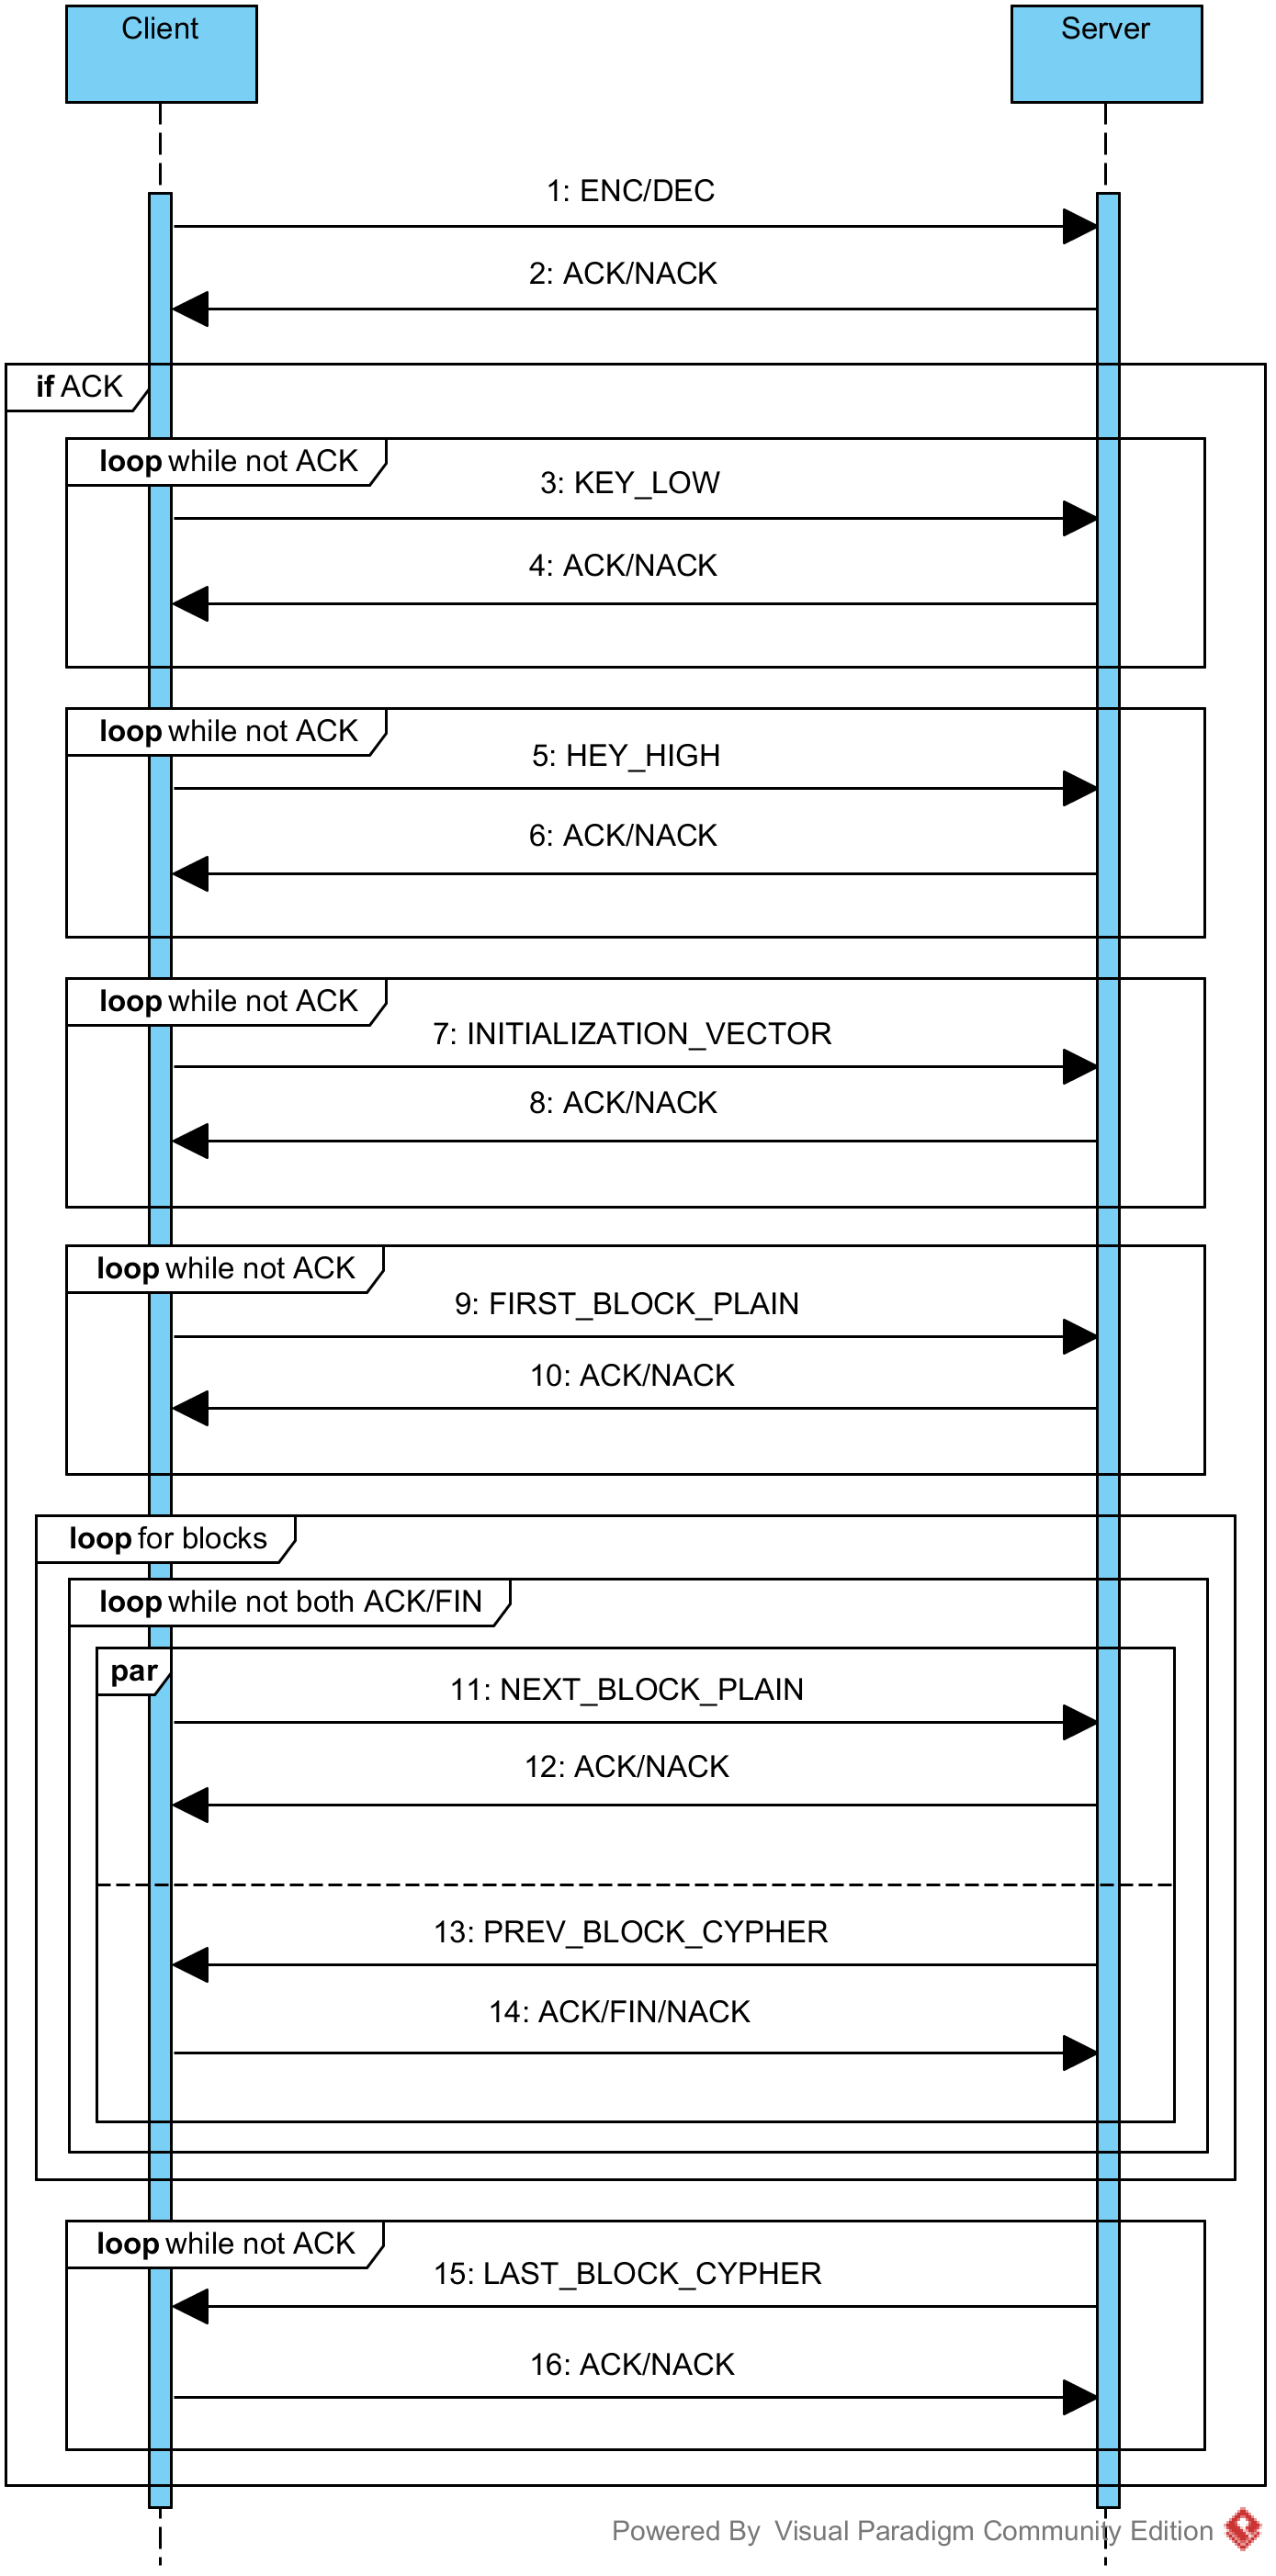
\includegraphics{pictures/communication-sequence.png}
\caption{Diagram sekwencji komunikacji między klientem a serwerem}
\label{fig:communication-sequence}
\end{figure}

Przebieg \ref{fig:communication-example} demonstruje przykład komunikacji w celu zaszyfrowania dwóch bloków danych, a schemat \ref{fig:communication-sequence} przestawia diagram sekwencji komunikacji między klientem i serwerem.

\newpage
\subsection{Struktura projektu FPGA}
Projekt, którym posłuży do zaprogramowania układu FPGA serwera podzielony jest na moduły (rys. \ref{fig:modules}):
\begin{description}
\item[\textit{communicator}] -- moduł odpowiedzialny za zarządzanie procesem przesyłania danych oraz szyfrowania lub deszyfrowania. Główną częścią modułu jest maszyna maszyna stanów (\textit{FSM}), która struje pozostałymi modułami.
\item[\textit{aes\_encryption}] -- moduł szyfrujący bloki AES.
\item[\textit{aes\_decryption}] -- moduł deszyfrujący bloki AES.
\item[\textit{uart\_rx}] -- moduł odbierający bajty.
\item[\textit{uart\_tx}] -- moduł wysyłający bajty.
\item[\textit{block\_serializer}] -- moduł formujący bloki AES ze strumienia odebranych bajtów.
\item[\textit{block\_deserializer}] -- moduł transformujący bloki AES w strumień bajtów do wysłania.
\item[\textit{MUX ENC/DEC}] -- selektor używany do przełączania trybu działania układu (szyfrowane / deszyfrowanie).
\item[\textit{MUX BLOCK/ACK}] -- selektor używany do przełączania źródła wysyłanych bajtów -- z modułu \textit{block\_serializer} (BLOCK) lub potwierdzeń odbioru (ACK).
\item[\textit{HPS}] -- komponent odpowiadający zintegrowanemu procesorowi ARM.
\end{description}

\begin{figure}[!h]
\centering
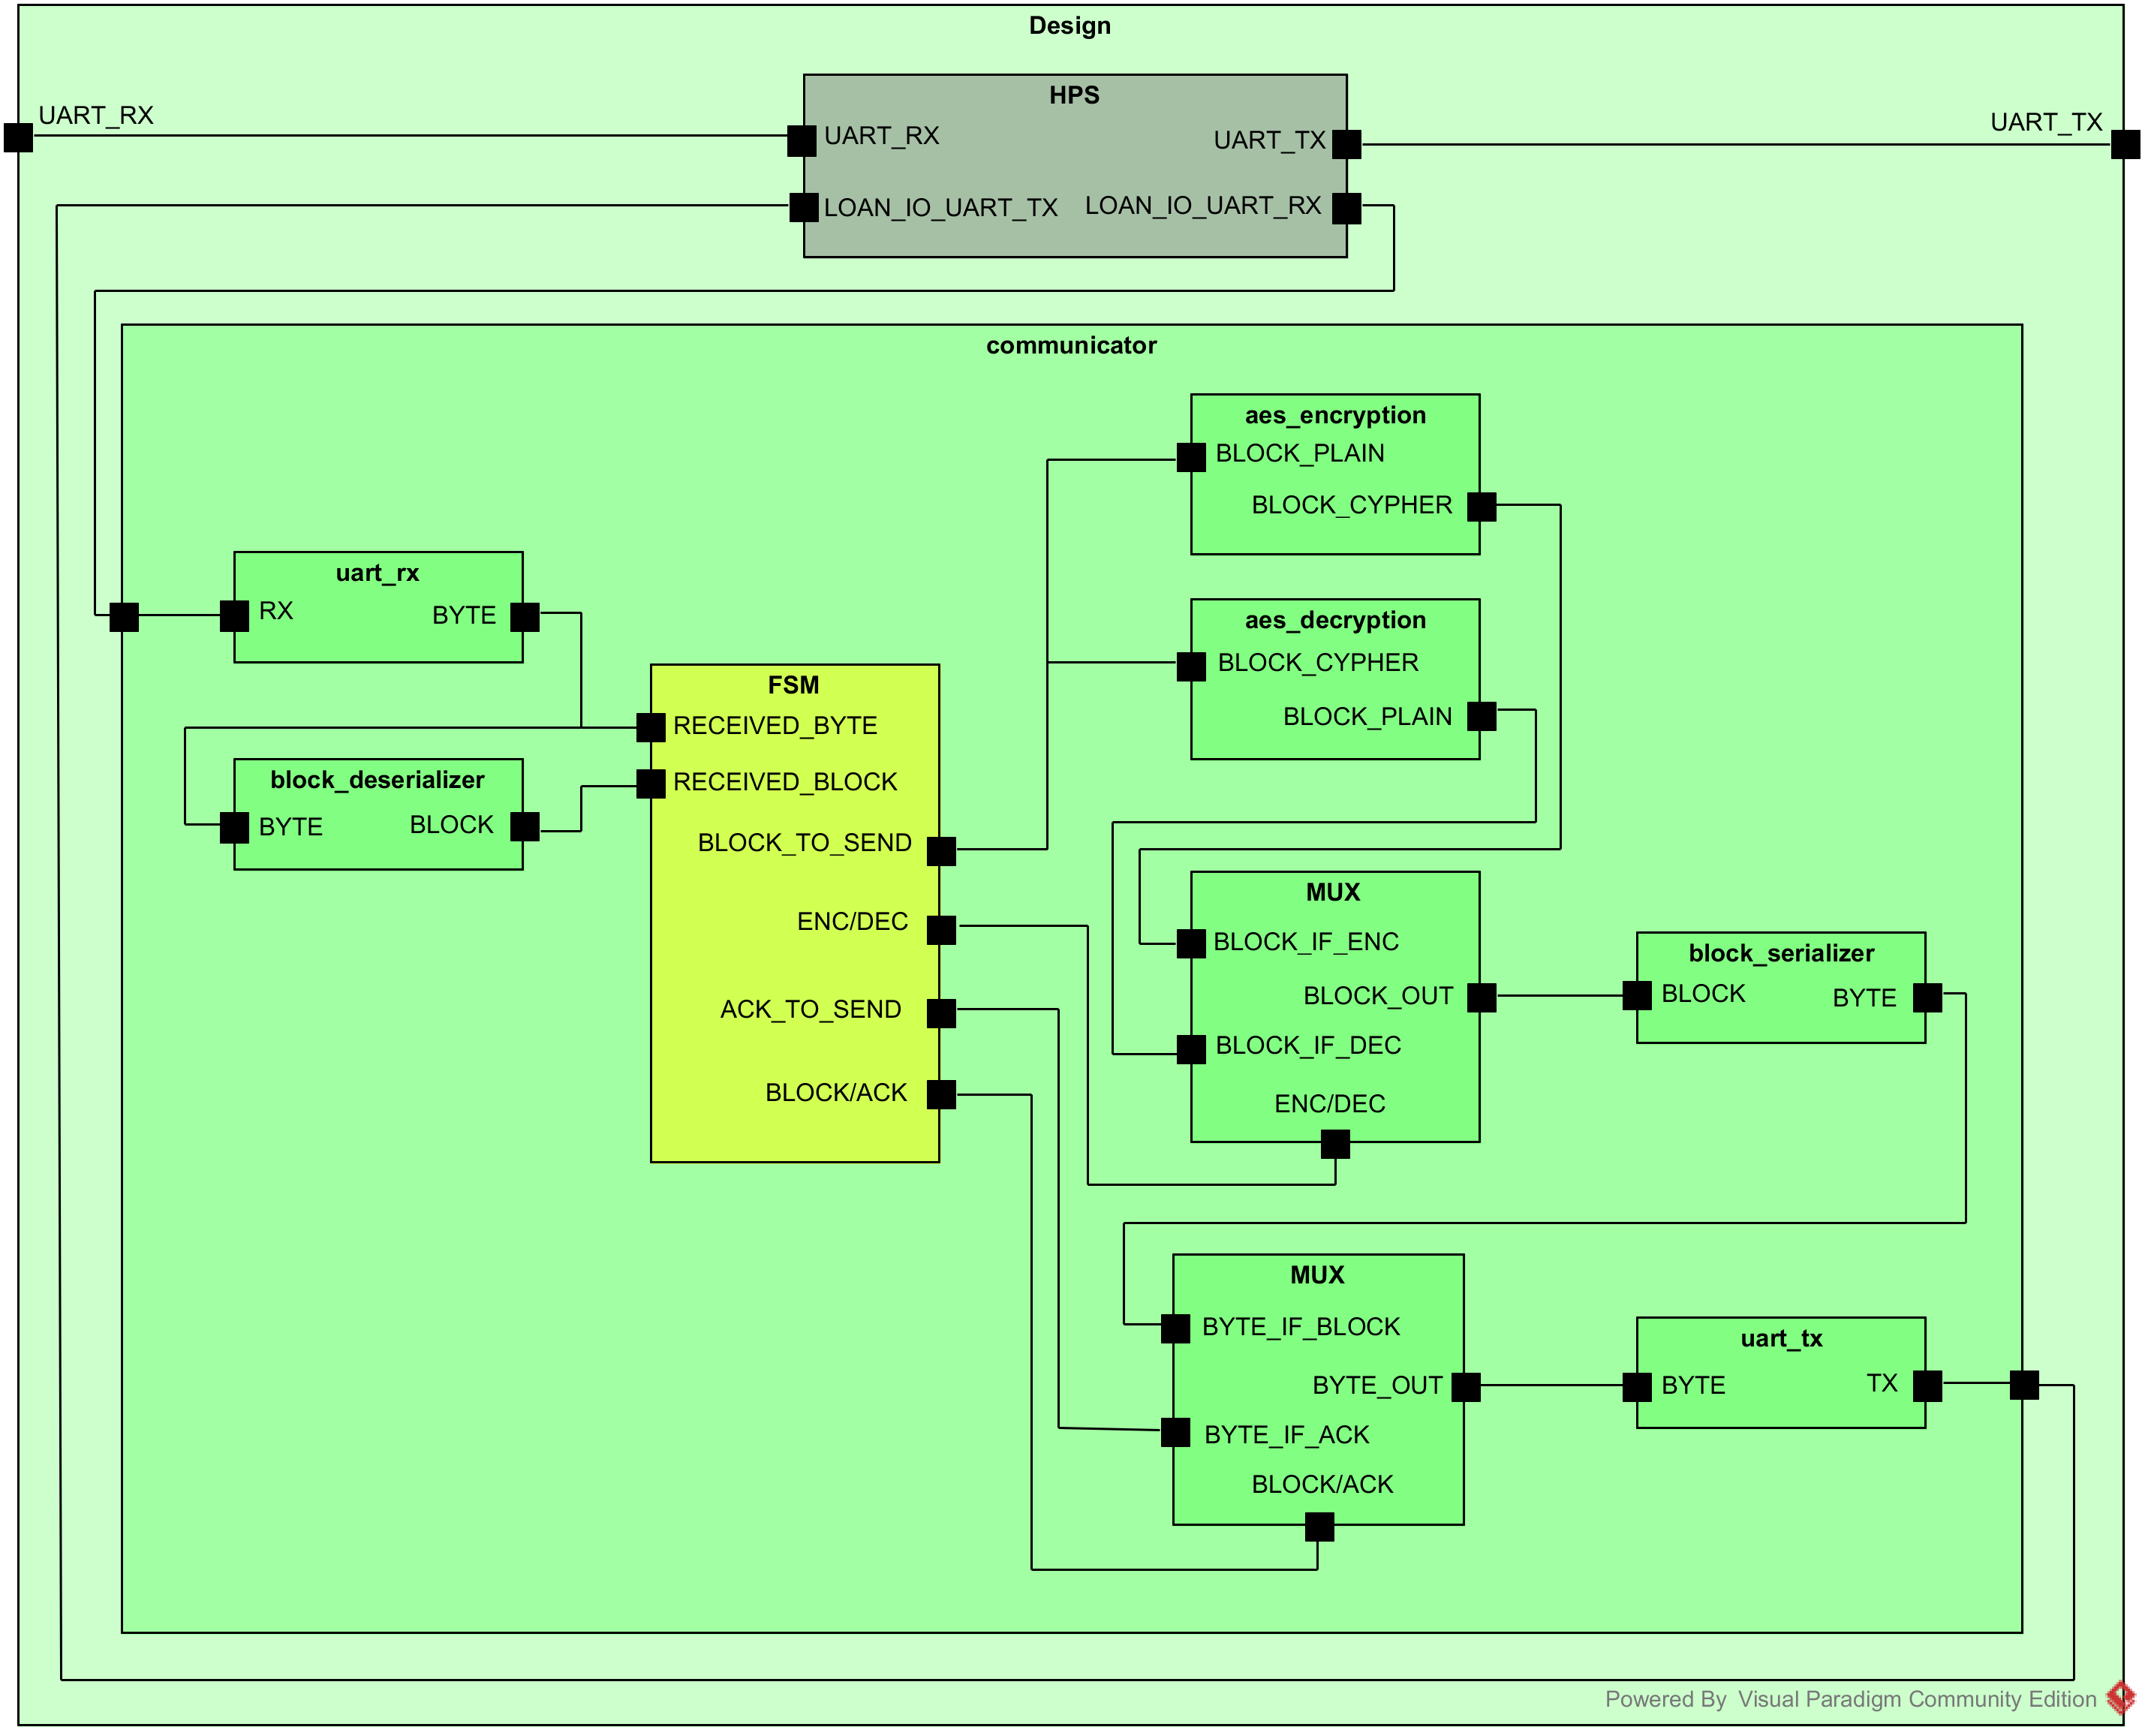
\includegraphics[width=\textwidth]{pictures/modules.png}
\caption{Schemat projektu FPGA}
\label{fig:modules}
\end{figure}

Wszystkie moduły wchodzące w skład projektu (rys. \ref{fig:modules}) są szczegółowo opisane w rozdziale \ref{sec:szczegoly-implementacyjne}.